
%% This file is based on bare_conf.tex
%% V1.4b
%% 2015/08/26
%% by Michael Shell
%% See:
%% http://www.michaelshell.org/
%% for current contact information.



\documentclass[conference]{IEEEtran}
\usepackage[utf8]{inputenc}
\usepackage{cite}
\usepackage{graphicx}
\usepackage{url}
\usepackage{todonotes}
%\usepackage{hyperref}
\usepackage{flushend}

\usepackage{glossaries}
\loadglsentries{acronyms}

% correct bad hyphenation here
\hyphenation{op-tical net-works semi-conduc-tor}


\begin{document}

%\title{\gls{oin}: A Free, Open Community \acrshort{IoT} Network based on \gls{lorawan}}
\title{A First Look At \gls{lorawan} Traffic Characteristics In Vienna's Community \acrshort{IoT} Network}

% author names and affiliations
% use a multiple column layout for up to three different
% affiliations
\author{\IEEEauthorblockN{Albert}
\IEEEauthorblockA{}
\and
\IEEEauthorblockN{Stefan}
\IEEEauthorblockA{}
}


% make the title area
\maketitle

%!TEX root = paper.tex
\begin{abstract}
The abstract goes here.
\end{abstract}


%!TEX root = paper.tex
\section{Introduction}


%!TEX root = paper.tex
\section{Overview}\label{sec-overview}

\gls{oin}, Vienna's community-operated \gls{IoT} network, hinges on
three architectural elements supporting its operation:
First, the wireless connectivity between sensors and the network
uses \gls{lora} and \gls{lorawan} specifically.
Second, the gateways and backend operate according to the architecture
proposed by \gls{ttn}~\cite{ttn}.
Third, gateways, backend, Internet connectivity etc. are built, operated,
maintained, and contributed by volunteer community members of \gls{oin},
all under the premise that the system is open to the public for use and
contributions on all layers.
In the following, we describe each aspect in greater detail.


\subsection{\gls{lora} and \gls{lorawan}}

\gls{lora} is a proprietary layer-1 technology for low-power long-range
low-bandwidth wireless transmissions. It operates in license-exempt
frequency ranges (the 433 MHz (EMEA, northern Asia) and 915 MHz
(the Americas) \acrshort{ISM} bands, and the European 868 MHz
\acrshort{SRD} band).



.... tech for l1/l2 ....



\subsection{\gls{ttn}'s system architecture}


\subsection{The \gls{oin} community}

%!TEX root = paper.tex
\section{Results}\label{sec:results}

Below we present first results from studying the aggregate
traffic across the multiple \gls{lorawan} gateways operated
by volunteers in the \gls{oin} community.
The current results were generated with an Elasticsearch-based
tool that focuses on selected and aggregated metrics.
\todo[inline]{Hier fehlt noch ein Satz über Kibana. Wer betreibt diese Instanz? Basiert sie auch auf TTN, oder ist das was eigenes?}
Thus, we
cannot yet report on metrics such as message inter-arrival times,
collisions, or the number of distinct senders. However, we
to extend the tool for more in-depth analysis in the future.

Our dataset aggregates more than two million messages seen between
mid-April and mid-May 2018 across 13 gateways in an area of around
250 square kilometers in and around Vienna, Austria.
The gateways operate in diverse locations, ranging from window sills
and rooftops of private homes to tall office and industrial buildings
across the hilly region of Vienna. Accordingly, the area of reception
varies greatly; maximum reception distances exceed 60 kilometers for
some gateways, while others mainly work in their close neighborhood.
Gateways also differ in terms of time deployed, their the hardware, and
frequency channels supported by it. Similarly, senders differ
in terms of output power and channel use, amounts of data generated,
mobility, etc.
With this caveat, we turn to discussing our first results.

\begin{figure}
  \centering
  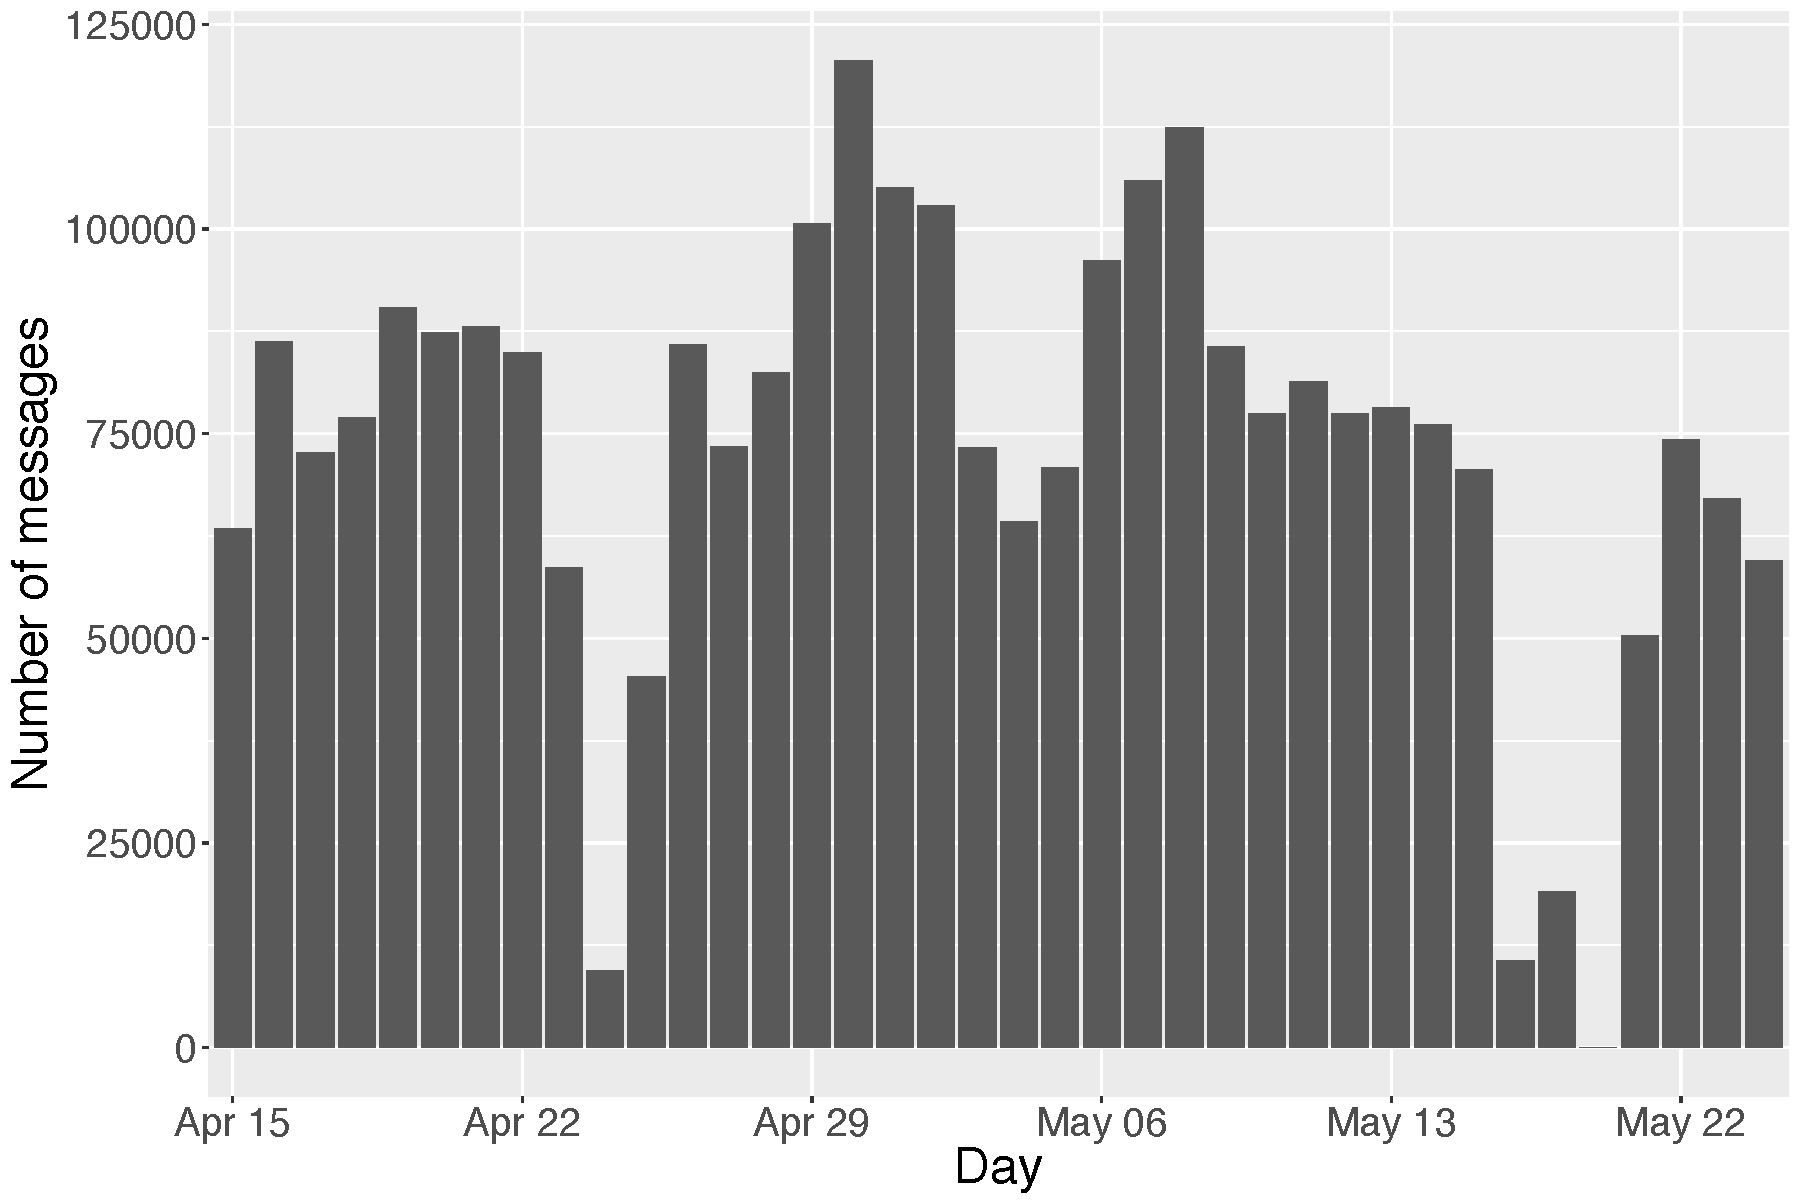
\includegraphics[width=\columnwidth]{figures/counts.pdf}
  \caption{Number messages per day across all gateways.}
  \label{fig:counts}
\end{figure}

Figure~\ref{fig:counts} shows the number of messages per day for the
evaluated period. The system handles an average (and median) of over
73,000 messages per day, with peaks up to 120,000, corresponding to
per-second averages of 0.8 and 1.3. A closer look reveals peaks
of up to 3 messages per second. The most ``popular'' gateway
receives 25\% of all messages; the three runners-up account for
the next 25\% of messages received.

\begin{figure}
  \centering
  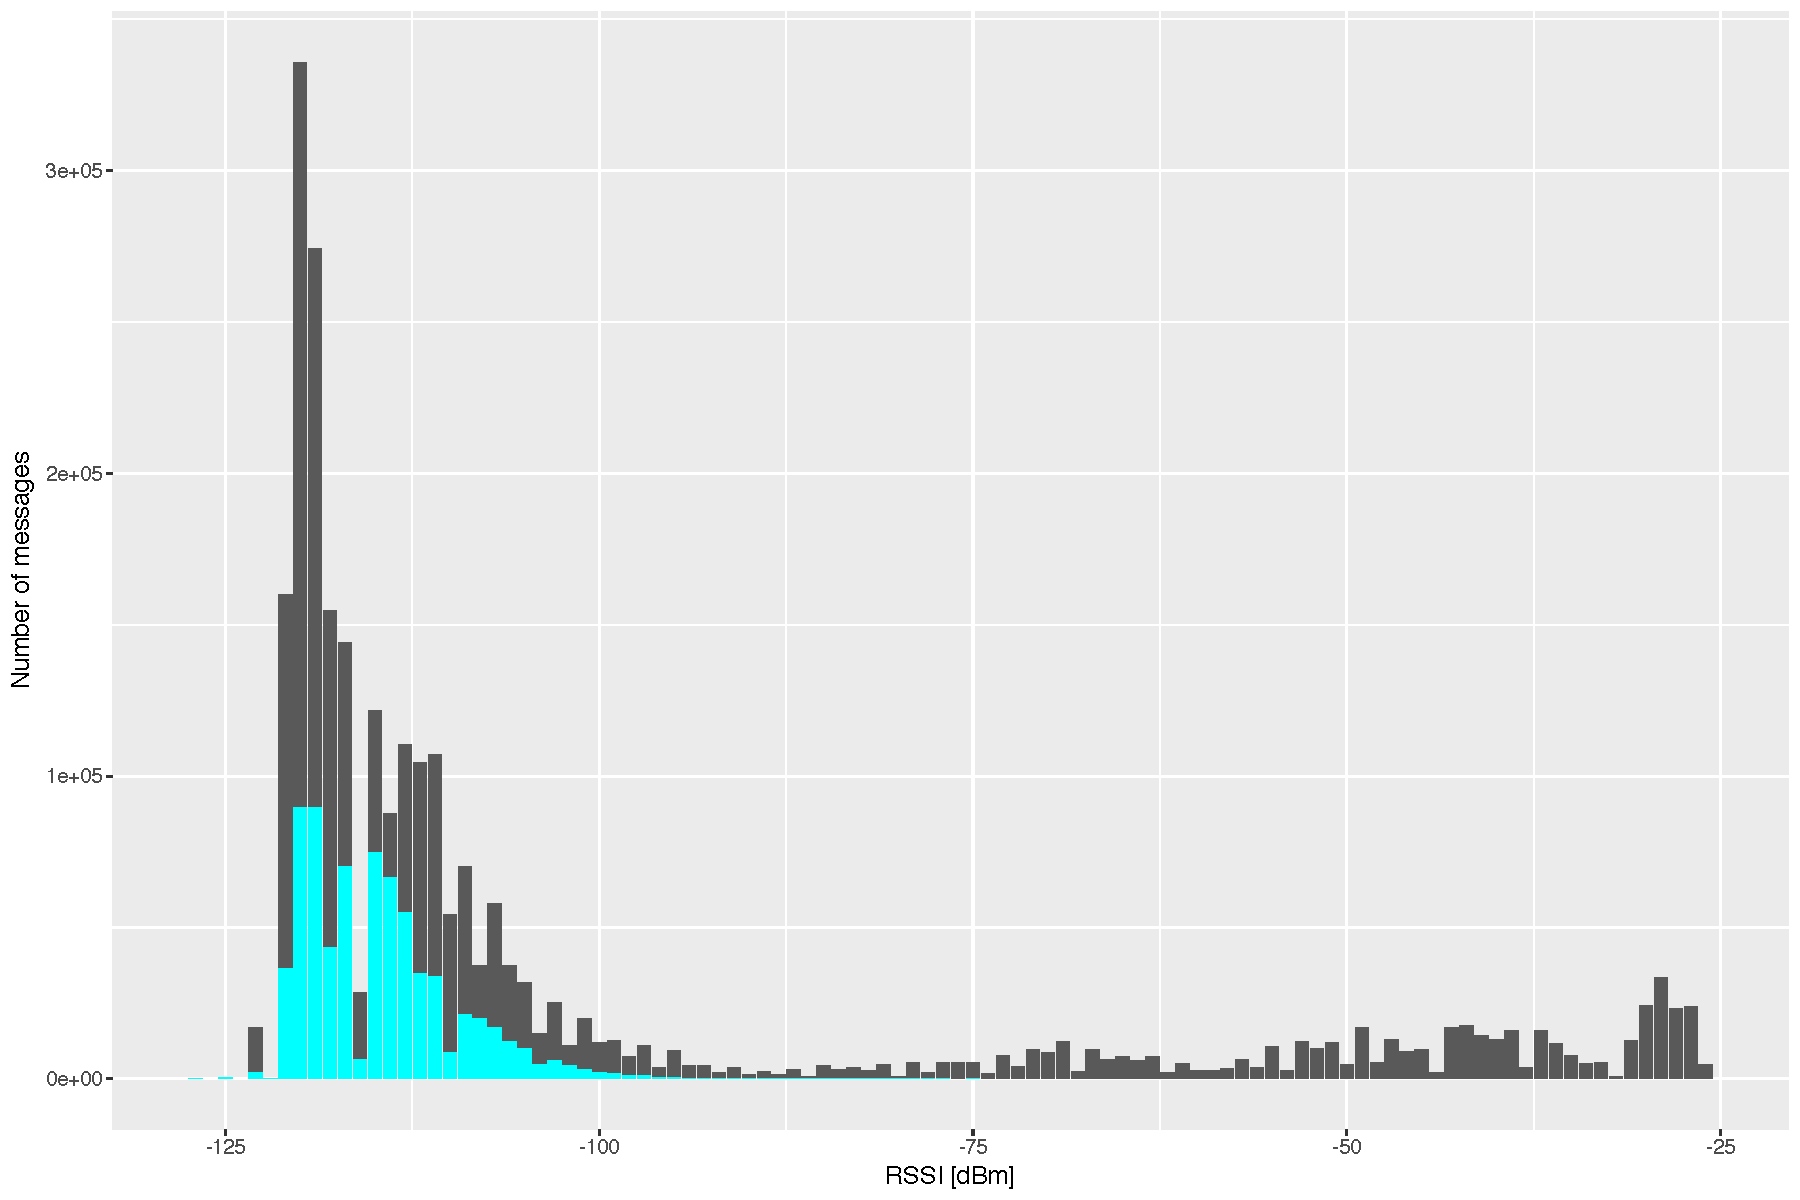
\includegraphics[width=\columnwidth]{figures/rssi.pdf}
  \caption{\acrshort{RSSI} for messages across all gateways (gray), and at the most active gateway (cyan).}
  \label{fig:rssi}
\end{figure}

Figure~\ref{fig:rssi} shows the \gls{RSSI} for messages across all
gateways (gray), and at the most active gateway (cyan).
\todo[inline]{keine geeichten Empfänger; wenig Leistung kommt an; Fading; Geografie der Empfänger; Geografie/Mobilität/nicht der Sender}




\begin{figure}
  \centering
  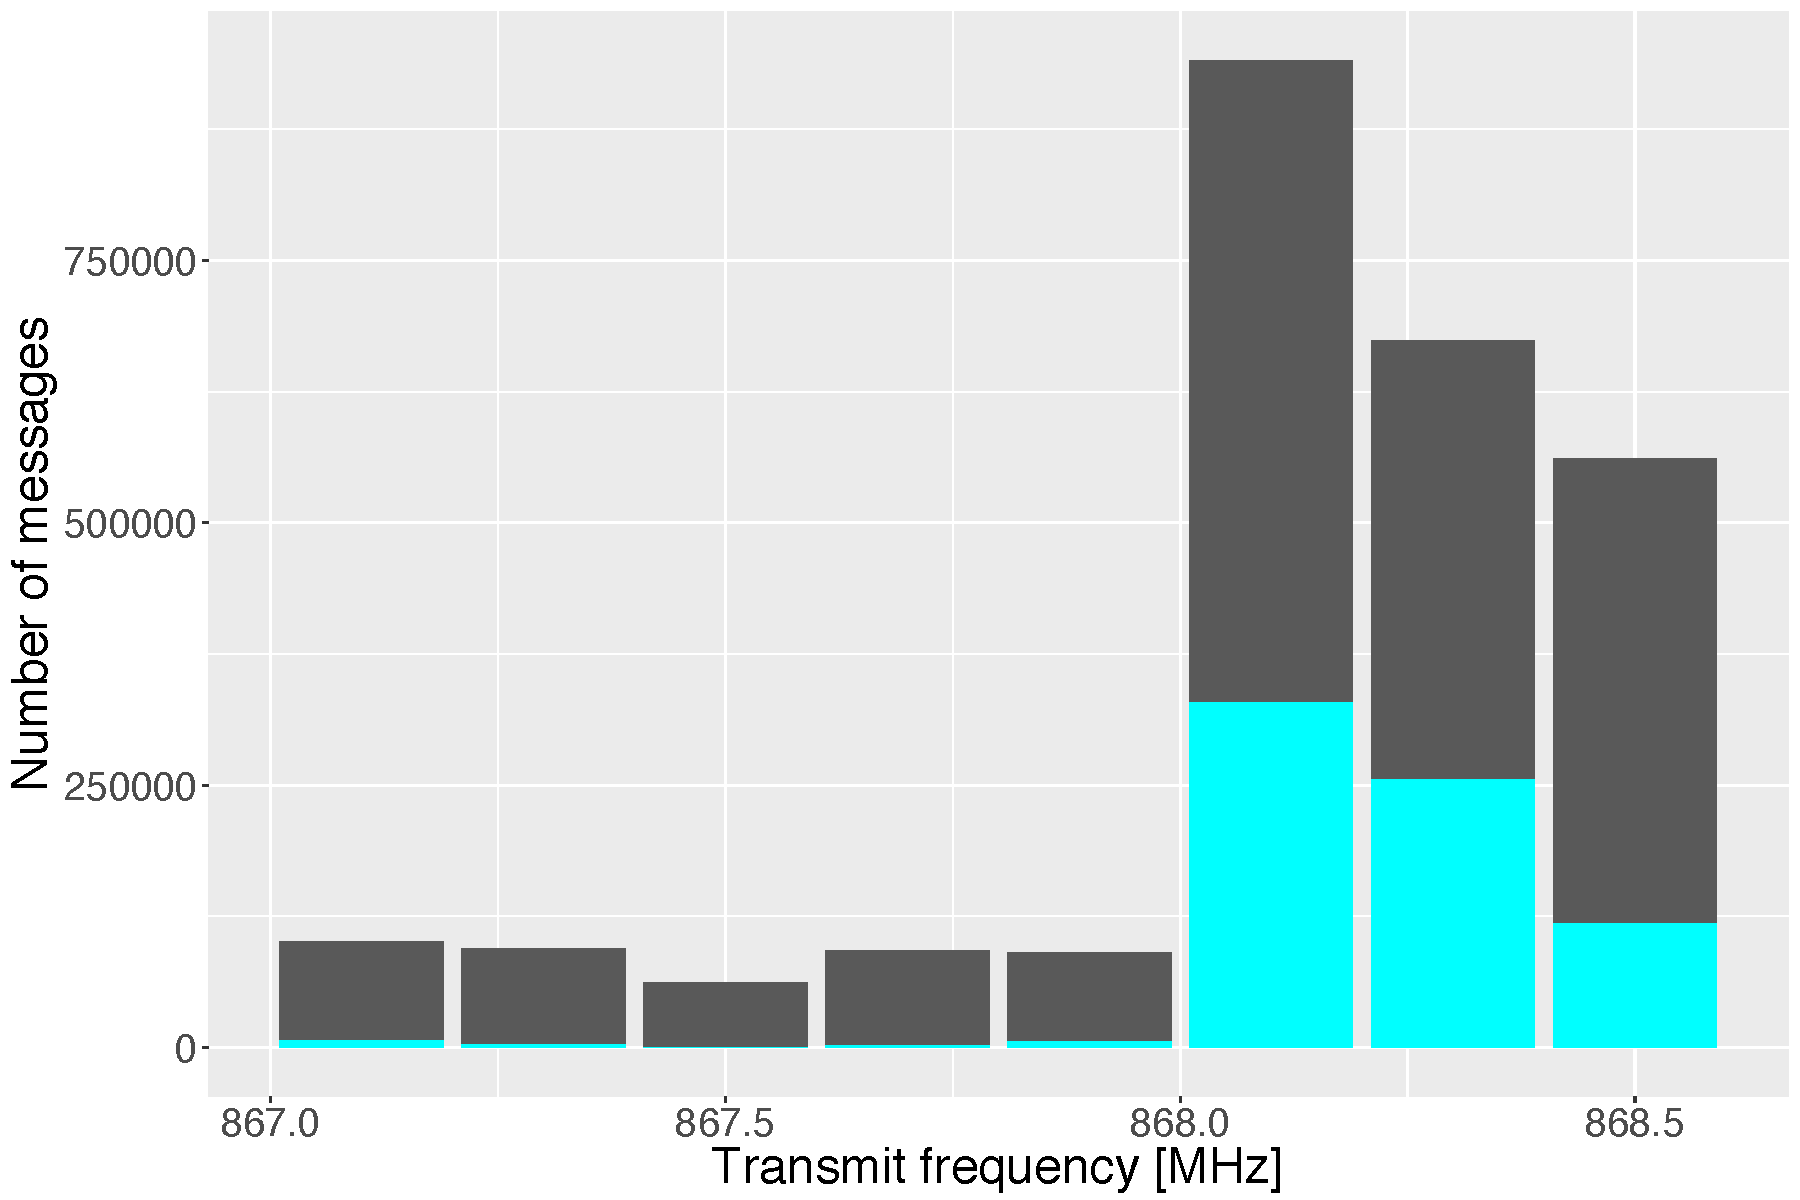
\includegraphics[width=\columnwidth]{figures/qrg.pdf}
  \caption{Transmission frequency for messages across all gateways (gray), and at the most active gateway (cyan).}
  \label{fig:qrg}
\end{figure}

Figure~\ref{fig:qrg} overviews the use of frequencies for transmissions
in the European \gls{SRD} band, as seen across all gateways (gray) and
at the most active gateway (cyan).
\todo[inline]{868,1 bis ,5 machen den Löwenanteil aus. Nicht alle Gateways können alle Frequenzen, und schon gar nicht alle Sender!}




\begin{figure}
  \centering
  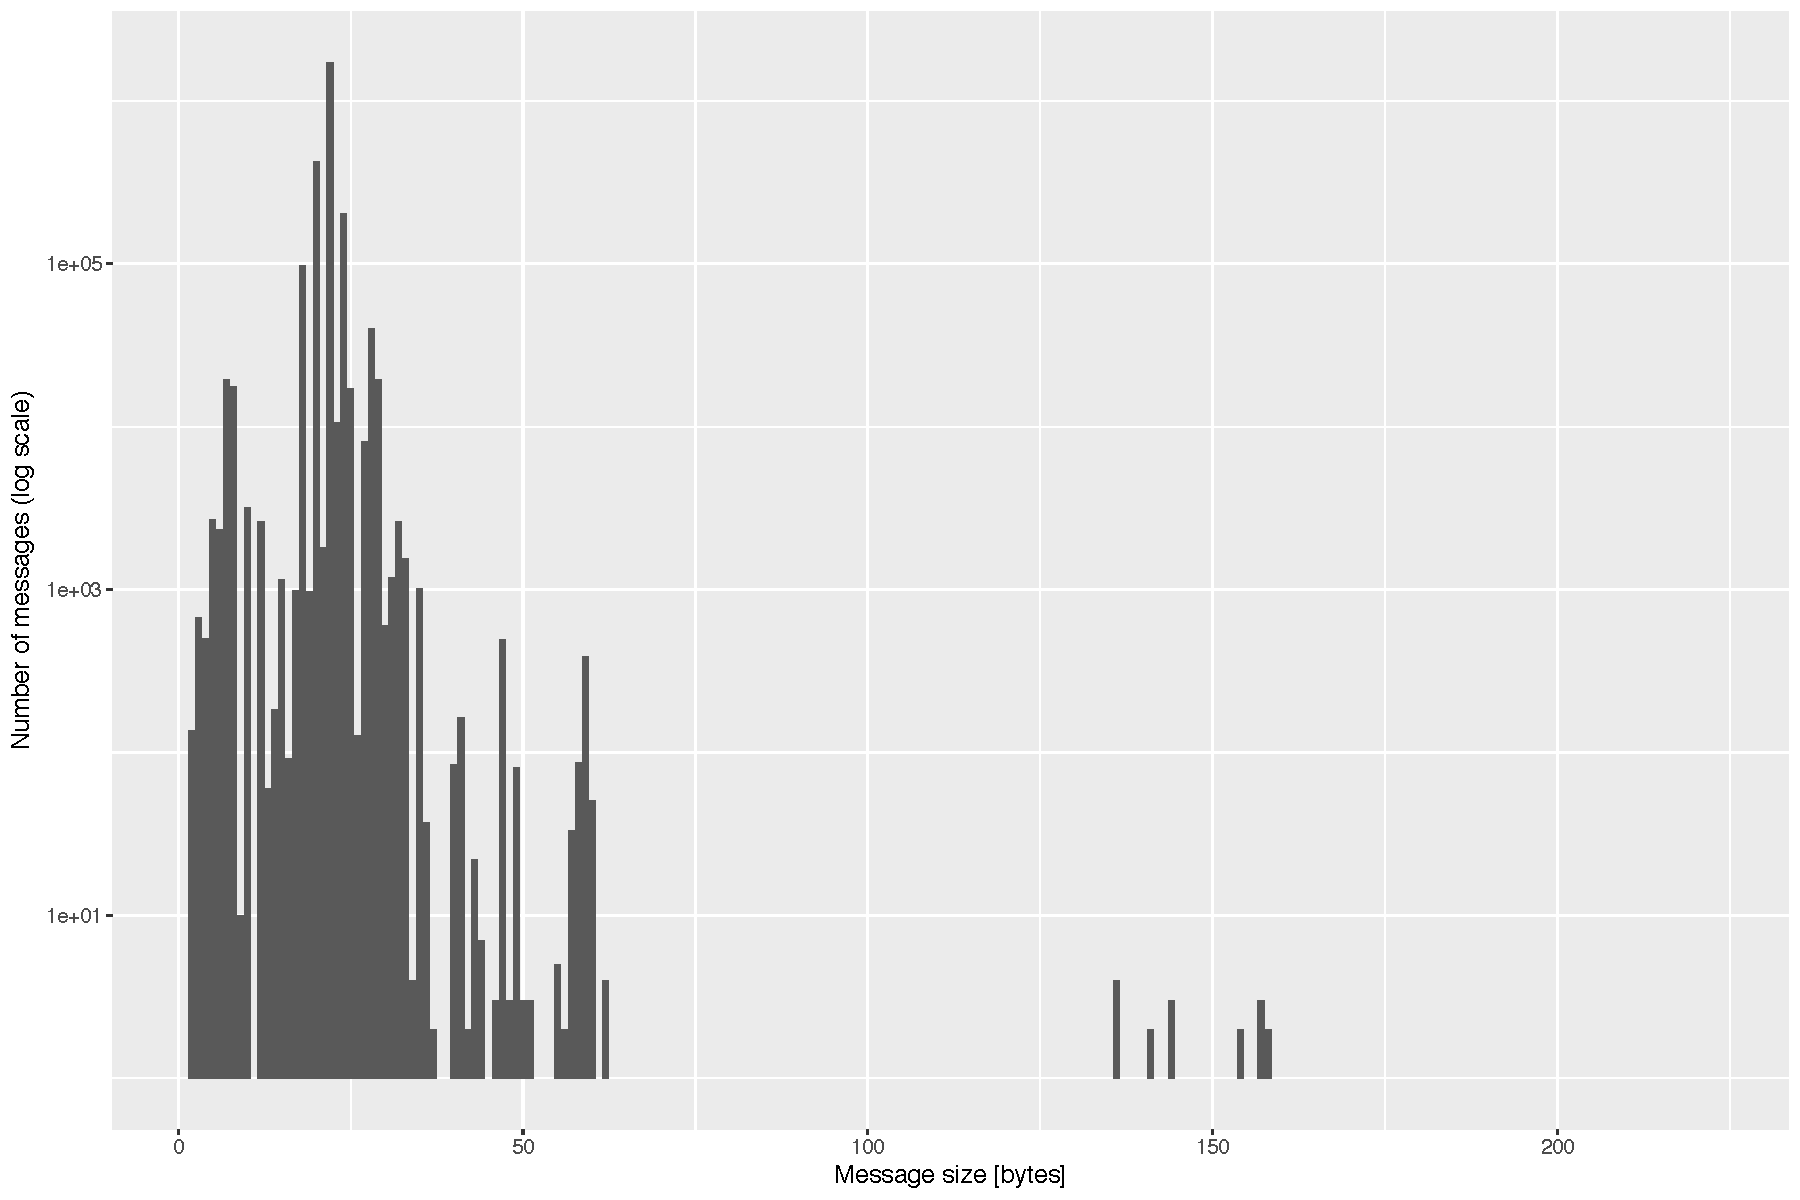
\includegraphics[width=\columnwidth]{figures/sizes.pdf}
  \caption{Message sizes across all gateways.}
  \label{fig:sizes}
\end{figure}

Figure~\ref{fig:sizes} plots the number of messages received across
all gateways, cumulated by message sizes. Note the logarithmic $y$ axis.
The mode of the distribution is $22$ bytes with a count of over 1.7 million.
A small cluster forms around the value.
\todo[inline]{Ein paar Spitzen (allerdings um Größenordnungen kleiner) gibt es noch; ohne detaillierten Blick in die Daten schwierig, weitere Schlüsse zu ziehen. Der prävalente SF12 ist immerhin kongruent mit kurzen Messages.}

%!TEX root = paper.tex
\section{Conclusion and Future Work}\label{sec:conclusion}

\todo[inline]{Zusammenfassung}

\todo[inline]{Bessere Auswertungen: IAT, pro Sender, Anonymisierung}
\todo[inline]{Aktives Mapping vs passiver Gateway-Blick. (Passiert natürlich schon, siehe ,,Messfahrten'')}
\todo[inline]{Daraus Modelle für Verkehr an Knoten, in der Aggregation; Spektrumnutzung}

%!TEX root = paper.tex
\section*{Acknowledgements}

openiot.network has been partially supported by ....

The first author has been supported by ....

The authors thank the openiot.network community.





% For peer review papers, you can put extra information on the cover
% page as needed:
% \ifCLASSOPTIONpeerreview
% \begin{center} \bfseries EDICS Category: 3-BBND \end{center}
% \fi
%
% For peerreview papers, this IEEEtran command inserts a page break and
% creates the second title. It will be ignored for other modes.
\IEEEpeerreviewmaketitle

\bibliographystyle{IEEEtran}
\bibliography{iot}


\end{document}

